\documentclass[letterpaper,10pt]{article}
\usepackage[top=2cm, bottom=1.5cm, left=1cm, right=1cm]{geometry}
\usepackage{amsmath, amssymb, amsthm,graphicx}
\usepackage{fancyhdr}
\pagestyle{fancy}

\lhead{\today}
\chead{MATH 710 Assignment 3}
\rhead{Justin Hood}

\newcommand{\Z}{\mathbb{Z}}
\newcommand{\Q}{\mathbb{Q}}
%\newcommand{\R}{\mathbb{R}}
\newcommand{\C}{\mathbb{C}}
\newcommand{\X}{$\textbf{X}$}
\newcommand{\eS}{$\textbf{S}$}
\newcommand{\Sn}{$\textbf{S}_n$}
\newcommand{\R}{$\textbf{R}$}
\newtheorem{lem}{Lemma}

\begin{document}
\begin{enumerate}
\item For this problem, we consider the dataset PSYCHPROFILE.DAT. A file containing 130 measurements from scores on a psychological test.
\begin{enumerate}
\item First, we construct our $\textbf{X}$ matrix. Given that we have $130$ observations of $5$ variables, our $\textbf{X}$ matrix will be $130\times 5$. Next, we compute our matrix of $\bar{x}$, the means of each variable. The results are,
\[\bar{x}'=\left[15.66923,\ 17.07692,\ 18.78462,\ 15.5,\ 11.73077\right]\]
Next, with these values in mind, we begin the construction of our \eS matrix. Our $\textbf{S}$ matrix is constructed using the formula,
\[s_{ik}=\frac{1}{n-1}\sum_{j=1}^n(x_{ji}-\bar{x}_i)(x_{jk}-\bar{x}_k)\]
From the size of \X , we know that the size of our \eS \ matrix should be, $5\times 5$. The resultant matrix is,
\[\textbf{S}=\begin{bmatrix}
34.750209 & -4.2766846 & -18.0717949 & -15.972868   & 5.716458\\
-4.276685 & 17.5134168   & 0.4197973  & -7.868217 &  -8.723315\\
-18.071795 &  0.4197973 &  29.8447227 &   9.348837 & -13.942159\\
-15.972868 &  -7.8682171 &   9.3488372  & 33.042636  & -9.941860\\
5.716458 &  -8.7233154 & -13.9421586 &   -9.941860 &   26.957961
\end{bmatrix} \]
Similarly, we compute our \R \ matrix from the $S$ matrix as,
\[r_{ik}=\frac{s_{ik}}{\sqrt{s_{ii}}\sqrt{s_{kk}}}\]
Thus,
\[\textbf{R}=\begin{bmatrix}
1.0000000 & -0.17335767 & -0.56116271 & -0.4713753  & 0.1867690\\
-0.1733577  & 1.00000000  & 0.01836202 & -0.3270797 & -0.4014696\\
-0.5611627  & 0.01836202  & 1.00000000  & 0.2977052 & -0.4915331\\
-0.4713753 & -0.32707967  & 0.29770524  & 1.0000000 & -0.3331093\\
0.1867690 & -0.40146956 & -0.49153305 & -0.3331093  & 1.0000000
\end{bmatrix} \]
We note, that as expected, we have $1$'s along the main diagonal.
\item Next, we consider the calculation of \Sn . We know that \eS is a bias corrected measurement of \textbf{$\Sigma$}, and has the form of,
\[\textbf{S}=\frac{n}{n-1}\textbf{S}_n\Rightarrow \textbf{S}_n = \frac{n-1}{n}\textbf{S}\]
So, since \Sn is $(129/130)$\eS , we may easily compute it,
\[\textbf{S}_n=\begin{bmatrix}
34.482899 & -4.243787 & -17.932781 & -15.850000 &  5.672485\\
-4.243787 & 17.378698   & 0.416568  & -7.807692  & -8.656213\\
-17.932781  & 0.416568  & 29.615148   & 9.276923 & -13.834911\\
-15.850000 & -7.807692   & 9.276923 &  32.788462  & -9.865385\\
5.672485 & -8.656213 & -13.834911  & -9.865385  & 26.750592
\end{bmatrix} \]
We see that this matrix is fairly close to our original computation of \eS , which makes sense, seeing as $129/130\approx 0.9923$. Given that \eS \ is computed with the bias correcting $n-1$ term, we will use it when dealing with sample vairance-covariance matrices. \Sn \ is computed in such a way that it more naturally falls out of the matrix definitions of these variable matrices. Using $\bar{x}$ to construct the deviation vectors, \Sn \ naturally falls out of basic matrix algebra. However, it is convenient that the conversion between the two is a simple scaling factor.
\item If we were to compute \R \ from \Sn \ instead of using \eS , we would obtain the same result. If we look at the equation for the entries of \R \ using \eS ,
\begin{align*}
r_{ik}&=\frac{s_{ik}}{\sqrt{s_{ii}}\sqrt{s_{kk}}}\\
&=\frac{\frac{1}{n-1}\sum_{ik}}{\sqrt{\frac{1}{n-1}\sum_{ii}}\sqrt{\frac{1}{n-1}\sum_{kk}}}\\
&=\frac{\sum_{ik}}{\sqrt{\sum_{ii}}\sqrt{\sum_{kk}}}
\end{align*}
Where in the above computation the sums of the differences to the mean have been condenced for brevity. A similar computation can be done using \Sn . Hence, we see that each term of the \R \ matrix does not depend on the scaling factor on the variance-covariance matrix, and will be the same regardless of which method used in the variance calculation.
\item We now consider an appropriate way to plot and compare these data sets. To begin, we look at the paired data plots, to see if there is any discernable correlations between the variables, to make sure our independence assumptions are valid.
\begin{center}
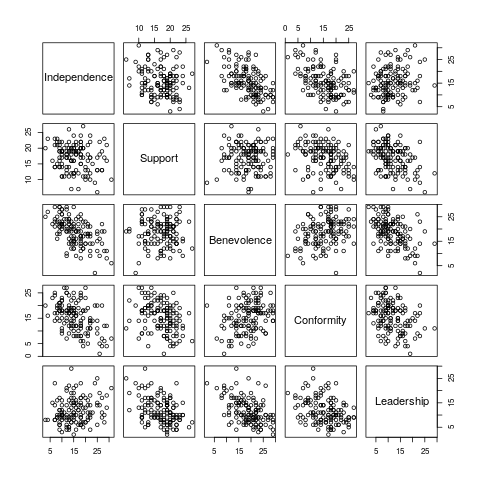
\includegraphics[scale=.7]{pairs.png}
\end{center}
In looking at this data, we see that there is not all that much correlation between the variables. We now also consider a boxplot of the data to compare the means and spreads of the different variables,
\begin{center}
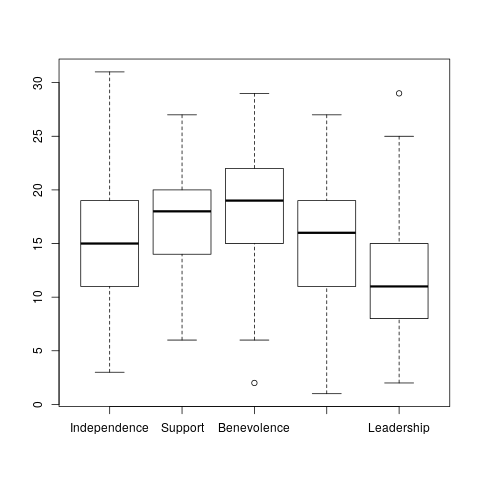
\includegraphics[scale=.65]{box.png}
\end{center}
We note that the IQR's for the different variables are all approximately equal, and appear to fall towards the center of the ranges in their data. We also see that the means of each of the variables are all somewhat close, this could be important to the researchers to know for their analysis.
\item Next, we consider each of the subscale scores for their marginal normality. To do this, we shall sort each of the variables in ascending order, along with the relative normal quantiles that correspond. Each variable is then assigned an $r_Q$ score, as a measurement of the correlation of their respective Q-Q plot. Finally, we test for normality, to determine if any of these variables violate our normal assumptions. Using $R$, we perform this analysis quickly, as well as plotting each of the Q-Q plots. Our results by variable follow,
\[r_Q=<0.9881301,\ 0.9892880,\ 0.9925086,\ 0.9933800,\ 0.9812888>\]
From a table, we note that the critical value of $r_Q$ for $n=130$ is, $r_Q^*=0.9873$ for $\alpha=0.05$. Our hypothesis test is then,
\[H_0: Normality,\ \ H_A: Non-Normal\]
Based on our test, we shall reject normality if our computed $r_Q$ value is less than that of our critical value. As such, we see that only one of our variables rejects our normal hypothesis, the Leadership variable. For completeness, find below the Q-Q plot of our independence (Left) and leadership variables (Right),
\begin{center}
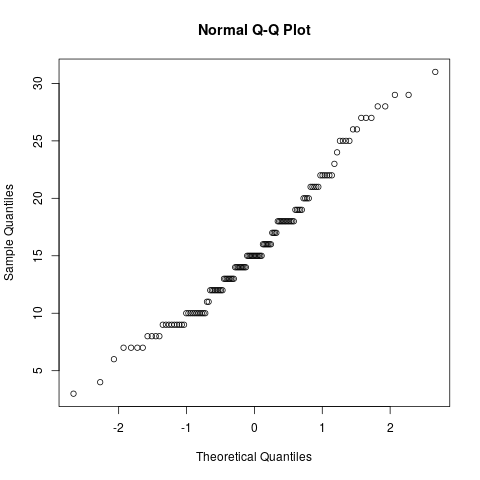
\includegraphics[scale=.5]{indepqq.png}
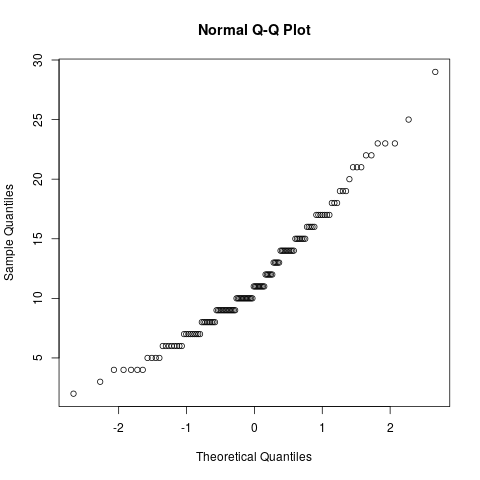
\includegraphics[scale=.5]{leaderqq.png}
\end{center}
We see that the curve for the leadership variable is slightly less straight than that of the independence variable, further confirming our conclusions about normality.
\item Given that our leadership variable is not normal, we consider how we might transform the data into a normal state. Using the Box-Cox method to transform the data, we consider values of $\lambda$ between $[-1,\ 1.5]$, where,
\[x^{(\lambda)}=\begin{cases}
\frac{x^{\lambda}-1}{\lambda} & \lambda \neq 0\\
\ln(x) & \lambda = 0
\end{cases} \]
Here, we are seeking to maximize the $\ell(\lambda)$ function. Using $R$, we compare different $\lambda$ values across the interval, incrementing by $0.01$. From this data, we see that the $\lambda$ value that maximizes our $\ell$ function is,
\[\lambda=0.38\]
So, we consider the new transformed variable,
\[LeadershipTransformed = \frac{Leadership^{0.38}-1}{0.38}\]
Performing our above Q-Q analysis on this value results in the new $r_Q$ value of,
\[r_Q=0.9964504\]
Which no longer violates our marginal normality test cutoff.
\item Next, we consider whether the data has a multivariate normal distribution. Based on the number of independent variables (5), we will expect that the overall data should exist within a $\chi^2_5$ distribution. As such, we consider the number of sample observations that lie within the ellipse,
\[(x-\bar{x})'S^{-1}(x-\bar{x})\leq \chi^2_5(0.5)\]
Using $R$, we solve for $S^{-1}$, and perform the above computation on each of the data points. We then compute the critical chi-square cutoff value for $50\%$, $\chi^2_5(0.5)=4.35146$. So, we are looking at points in $X$ that have a squared distance value less than $4.35146$. From our computations, we see that only $13$ values are within this cutoff, or $10\%$. If this were truly from a multivariate normal distribution, we would expect approximately 50\% of the data to fall within the ellipse. Next, we construct a Chi-Square plot of the distances,
\begin{center}
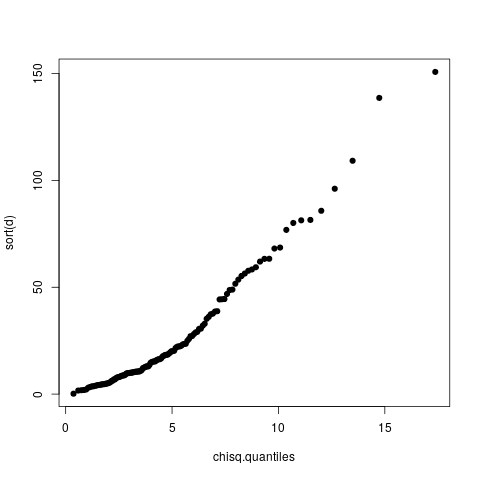
\includegraphics[scale=.7]{psychchi.png}
\end{center}
On the surface, this plot seems fairly linear, however, the slope is not 1, it is approximately 10. This is another violation of our normality conditions. Thus, we conclude that these subscores are not from a multivariate normal distribution.
\item Finally, we consider adding a column to the data that consists of an ``overall" score, which is computed by averaging the values of each subscale scores. From with this new data, we consider what the new $\bar{x}$ and \eS \ matrixes will be. From experience, we know that the new $\bar{x}$ matrix will be the mean of the old $\bar{x}$ matrix, or,
\[\bar{x}=15.75231\]
The variance matrix is slightly more complex, but the new \eS \ matrix will be the mean of all the entris in the old \eS \ matrix, or,
\[\textbf{S} = 0.6194132\]
\end{enumerate}
\item Given that a matrix $A$ is symmetric, and of size $p\times p$ where $p\geq 2$, we see that $A$ is positive definite iff the leading principle submatrix is positive definite, and $|A|>0$. So, we consider,
\[\Sigma=\begin{bmatrix}
19254770 & 9644284 & 31090422\\
9644284 & 78716208 & 32475410\\
31090422 & 32475410 & 77679998
\end{bmatrix}\]
\begin{enumerate}
\item Partitioning as described, we arrive at the following components,
\begin{align*}
A_* &= \begin{bmatrix}
19254770 & 9644284\\
9644284 & 78716208
\end{bmatrix}\\
a &= \begin{bmatrix}
31090422\\32475410
\end{bmatrix}\\
c &= 77679998
\end{align*}
First, we must test to see if $A_*$ is positive definite. Given that $A_*$ is of order (2x2), we recursively compute with our theorem to test if it is positive definite. Now,
\begin{align*}
A_{*_*} &= 19254770\\
a_* &= 9644284\\
c_* &= 78716208
\end{align*}
So, we see that $A_{*_*}$ is positive definite, and $|A_*|=1.42265e+15>0$. So $A_*$ is positive definite. Now, we consider the determinant of $|\Sigma|$. Using $R$ we compute the determinant to be, $3.359134e+22>0$. So, since $A_*$ is positive definite, and $|\Sigma|>0$, we conclude that $\Sigma$ is positive definite.
\item Another method for testing whether $\Sigma$ is positive definite is to compute the eigenvalues. If all eigenvalues are positive, the matrix is positive definite. Using $R$, we compute the eigenvalues to be,
\[\lambda =119184544,\  50932807,\   5533625\]
Which are all greater than zero. Thus, we see that $\Sigma$ is positive definite.
\end{enumerate}
\item We consider the matrix,
\[A=\begin{bmatrix}
9 & -2\\-2 & 6
\end{bmatrix} \]
\begin{enumerate}
\item To compute the inverse of a $(2\times 2)$ matrix, we first compute,
\[|A|=9(6)-(-2(-2))=50\]
The inverse of $A$ is then,
\[A^{-1}=\frac{1}{50}\begin{bmatrix}
6 & 2\\2 & 9
\end{bmatrix}=\begin{bmatrix}
0.12 & 0.04\\ 0.04 & 0.18
\end{bmatrix} \]
\item We now compute the following,
\[(A-\lambda I)=0\]
This becomes,
\begin{align*}
0 &= \begin{vmatrix}
6-\lambda & -2\\-2 & 9-\lambda
\end{vmatrix}\\
&=(6-\lambda)(9-\lambda)-(-2)(-2)\\
&=\lambda^2-15\lambda+50\\
\lambda &= 5,\ 10
\end{align*}
We then consider the eigenvectors associated with these values,
\begin{align*}
\lambda_1=5 &\Rightarrow \begin{bmatrix}
9-5 & -2\\-2 & 6-5
\end{bmatrix}\\
&=\begin{bmatrix}
4 & -2\\ -2 & 1
\end{bmatrix}\\
&= \begin{bmatrix}
2 & -1\\ 0 & 0
\end{bmatrix}
\end{align*}
This results in the equation,
\[2x_1-x_2=0 \Rightarrow 2x_1=x_2\]
Thus, our eigenvector is,
\[e_1 = \begin{bmatrix}
1\\2
\end{bmatrix}\]
With the other eigenvalue,
\begin{align*}
\lambda_1=5 &\Rightarrow \begin{bmatrix}
9-10 & -2\\-2 & 6-10
\end{bmatrix}\\
&=\begin{bmatrix}
-1 & -2\\ -2 & -4
\end{bmatrix}\\
&= \begin{bmatrix}
1 & 2\\ 0 & 0
\end{bmatrix}
\end{align*}
This results in the equation,
\[x_1+2x_2=0 \Rightarrow x_1=-2x_2\]
Thus, our eigenvector is,
\[e_2 = \begin{bmatrix}
-2\\1
\end{bmatrix}\]
\item To compute the spectral decomposition of $A$, we first normalize the eigenvectors,
\[e_1=\begin{bmatrix}
\frac{1}{\sqrt{5}}\\\frac{2}{\sqrt{5}}
\end{bmatrix},\ e_2=\begin{bmatrix}
\frac{-2}{\sqrt{5}}\\\frac{1}{\sqrt{5}}
\end{bmatrix} \]
Our decomposition is then,
\begin{align*}
A &= \lambda_1e_1e_1'+\lambda_2e_2e_2'\\
&=5\begin{bmatrix}
\frac{1}{\sqrt{5}}\\\frac{2}{\sqrt{5}}
\end{bmatrix}\begin{bmatrix}
\frac{1}{\sqrt{5}} & \frac{2}{\sqrt{5}}
\end{bmatrix}+10\begin{bmatrix}
\frac{-2}{\sqrt{5}}\\\frac{1}{\sqrt{5}}
\end{bmatrix}\begin{bmatrix}
\frac{-2}{\sqrt{5}} & \frac{1}{\sqrt{5}}
\end{bmatrix}\\
&=5 \begin{bmatrix}
1/5 & 2/5 \\
2/5 & 4/5
\end{bmatrix}+10\begin{bmatrix}
4/5 & -2/5\\
-2/5 & 1/5
\end{bmatrix}\\
&=\begin{bmatrix}
1 & 2\\
2 & 4
\end{bmatrix}+\begin{bmatrix}
8 & -4\\
-4 & 2
\end{bmatrix}\\
&=\begin{bmatrix}
9 & -2\\
-2 & 6
\end{bmatrix}
\end{align*}
\end{enumerate}
\item We consider the matrices,
\[A=\begin{bmatrix}
4 & 4.001\\
4.001 & 4.002
\end{bmatrix},\ B=\begin{bmatrix}
4 & 4.001\\
4.001 & 4.002001
\end{bmatrix} \]
\begin{enumerate}
\item We compute $A^{-1}$ and $B^{-1}$ as follows,
\[|A|=4(4.002)-4.001^2=16.008-16.008001=-0.000001\]
\[|B|=4(4.002001)-4.001^2=16.008004-16.008001=-0.000003\]
Our inverses are then,
\[A^{-1}=\frac{1}{-1\times10^{-6}}\begin{bmatrix}
4.002 & -4.001\\-4.001 & 4
\end{bmatrix}=\begin{bmatrix}
-4002000 & 4001000\\ 4001000 & -4000000
\end{bmatrix} \]
\[B^{-1}=\frac{1}{-3\times10^{-6}}\begin{bmatrix}
4.002001 & -4.001\\-4.001 & 4
\end{bmatrix}=\frac{1}{3}\begin{bmatrix}
-4002001 & 4001000\\
4001000 & -4000000
\end{bmatrix}\]
We see that the differences between the two inverses are different by almost exactly a factor of $3$.
\item We consider why the difference is so extreme, given the minute difference between the last entry in the two matrices. Consider the inverse formula,
\[A^{-1}=\frac{1}{det(A)}adj(A)\]
Because the determinant is of the order $c\times 10^{-6}$, we see that our inverse formula becomes,
\[A^{-1}=\frac{10^6}{c}adj(A)\]
This small determinant actually scales the elements of the $adj(A)$ matrix by a large order of magnitude. Then, our $c$ value has a more powerful effect on the overall result than one might consider. Here, our difference had $c=3$, and the resultant matrix was scaled by a factor of $3$, with elements of magnitude $10^6$.
\end{enumerate}
\item We consider the EQI variables from the data file. 
\begin{enumerate}
\item As before, we compute $\bar{\textbf{x}},\ \textbf{S},\ \textbf{R}$. The results are,
\[\bar{\textbf{x}}=[3.024514e-09,\ -1.942057e-09,\ 4.317096e-09,\ 2.54696e-10,\ 6.017192e-09,\ -3.502069e-10]\]
These means are all very close to zero. We then compute the $\textbf{S}$ and $\textbf{R}$ matrices as,
\[\textbf{S}=\begin{bmatrix}
1.00000001 & 0.08063537 & 0.09181849 & 0.3760504 & 0.3999410 & 0.6791323\\
0.08063537 & 1.00000001 & 0.17506718 & 0.1118162 & 0.1591609 & 0.3652640\\
0.09181849 & 0.17506718 & 0.99999999 & 0.3389801 & 0.1896861 & 0.5423262\\
0.37605042 & 0.11181622 & 0.33898013 & 1.0000000 & 0.3192387 & 0.7458523\\
0.39994097 & 0.15916089 & 0.18968611 & 0.3192387 & 1.0000000 & 0.7083763\\
0.67913225 & 0.36526401 & 0.54232619 & 0.7458523 & 0.7083763 & 1.0000000
\end{bmatrix}\]
\[\textbf{R}=\begin{bmatrix}
1.00000000 & 0.08063537 & 0.09181849 & 0.3760504 & 0.3999410 & 0.6791323\\
0.08063537 & 1.00000000 & 0.17506718 & 0.1118162 & 0.1591609 & 0.3652640\\
0.09181849 & 0.17506718 & 1.00000000 & 0.3389801 & 0.1896861 & 0.5423262\\
0.37605041 & 0.11181622 & 0.33898013 & 1.0000000 & 0.3192387 & 0.7458523\\
0.39994097 & 0.15916089 & 0.18968611 & 0.3192387 & 1.0000000 & 0.7083763\\
0.67913225 & 0.36526400 & 0.54232620 & 0.7458523 & 0.7083763 & 1.0000000
\end{bmatrix} \]
We see that our \R \ and \eS \ matrices are nearly identical. This is due to the ``$1$'s" on the diagonal of the $S$ matrix.
\item We now compute the generalized variances for each of the states, AL, CA, CT, WI. As a test, we first consider the generalized variance of $\textbf{S}$.
\[|\textbf{S}|=2.238467e-14\approx 0\]
So, based on a zero generalized variance, we see that one of the columns is a linear combination of the others. So, let us consider the eigenvalues of the matrix. There is one eigenvalue that is approximately zero, with corresponding eigenvector,
\[e=<-0.2835367,\ -0.1524972,\ -0.2264204,\ -0.3113923,\ -0.2957461,\  0.8128065>\]
So, we see that the last column of the data can be expressed as the linear combination of the rest of the data points, and is hindering our variance computations. So, for our computations with the four states, we shall ignore the last EQI column to avoid the redundancy. Partitioning the data by state, and computing the generalized variance for each, we see the following,
\begin{align*}
|AL| &= 4.435441e-04\\
|CA| &= 6.687107e-04\\
|CT| &= 1.090844e-07\\
|WI| &= 1.573860e-03
\end{align*}
Here, we see that the generalized variances are small, but now much more distinct. Because generalized variance is a singular value measurement about the spread of the data in $p$ space, these values tell us about how the environmental quality of each of these states is grouped. Sorting in order from least to greatest, we arrive at, $CT\to AL\to CA\to WI$. Meaning, that across the entire state of Connecticut, the overall environmental quality only varies slightly, while compared to Wisconsin, the quality varies far more across the state. This however does not necessarily take into account the relative sizes of the states, among other factors, and should not be taken as truth without due consideration.
\item Now, we partition the values of Nevada by county and compare the correlations between them. The variable $C$ contains the correlation matrix in $R$, and a plot of the relative correlations follows,
\begin{center}
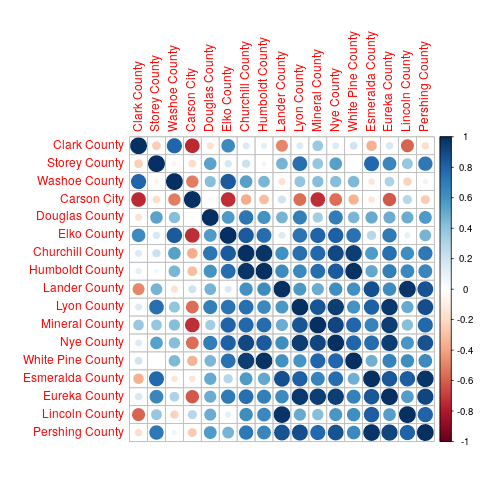
\includegraphics[scale=1]{corr.png}
\end{center}
Before we computed this correlation, we ranked the different counties from highest urbanized to thinnest population $(Left\to Right)$ and $(Top\to Bottom)$ in the above graphic. What we see from this data is that the correlations between the less populated counties are higher then when compared to the higher urbanized parts of the state. This makes sense, as the lesser populated counties should all have a similar environmental status, as less human randomness is introduced into the area.
\item Finally, as before, we consider whether the EQL variables are marginally distributed normally. For each variable, we compute the $r_Q$ coefficient and compare it to our critical value. From the text, we only know that for $n=300$ the cutoff is $0.9953$. For our EQI data, we are dealing with over $3000$ different observations. As such, we know that our critical cutoff would be higher. Comparing the $r_Q$ values to the cutoff, we find that none of the variables have a high enough score to be conisdered normal. Looking at the QQ plots, here are the highest and lowest $r_Q$ scored variables, $Socio=0.9951913$ (left) and $Land=0.8998543$ (right).
\begin{center}
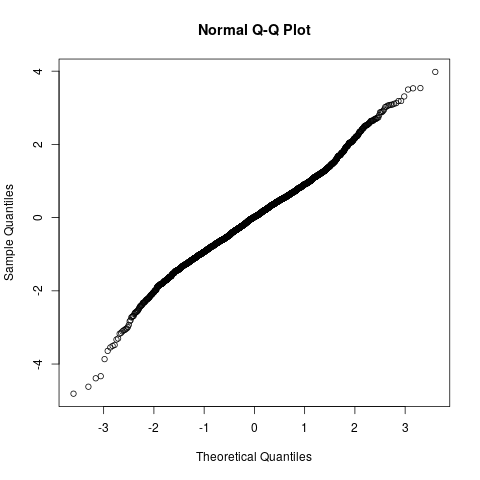
\includegraphics[scale=.5]{highqq.png}
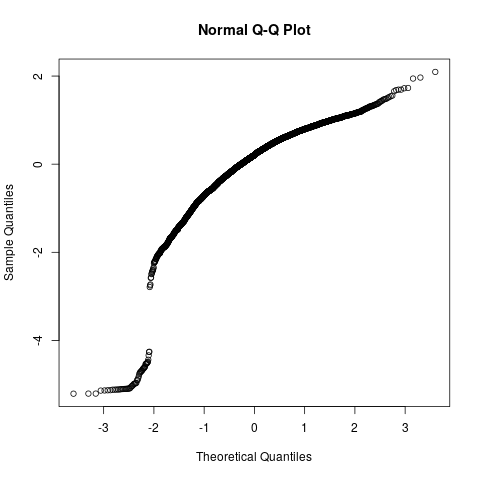
\includegraphics[scale=.5]{lowqq.png}
\end{center}
We see that the socio variable is nearly linear, so it is very close to normal, while the land variable is not very linear at all, indicating low normalcy.
\end{enumerate}
\end{enumerate}
\end{document}
